\documentclass[10pt]{article}
\usepackage{icmlko}

\icmlmeta{IP 파운데이션 월드모델}{96}{없는 축이 돕는다}{임베딩의 첫 성분은 길이였는데, 그 축을 출처에 붙일 때마다 축이 없는 팝업이 출처 하나당 $+$0.0035씩 올랐다}

\begin{document}

\twocolumn[
\icmlheader

\begin{abstract}
노트 95가 두 가지를 남겼다 --- 겹침 56\%가 무엇끼리인지 안 갈랐고, 손 특징
다섯 대신 임베딩을 안 뽑았다. 둘 다 했다. \textbf{겹침은 새 축끼리가 아니었다}
--- 직전작 성적과 문장 수의 상관은 다섯 도메인 중 셋에서 0.03 아래고, 대신
\textbf{둘 다 기존 다섯 축과 겹친다}(직전작 $\leftrightarrow$ 모바일 입장료
$-$0.495, 문장 수 $\leftrightarrow$ 타깃 폭 $+$0.13$\sim+$0.20). 임베딩은 문자
2--4 그램 TF-IDF 60,000차원을 SVD 로 줄여 만들었다(모형 없이, 12,103건).
\textbf{첫 성분은 길이였다} --- 손 특징 ``문자 수''와 $+$0.47$\sim+$0.82로
붙는다. 축으로 넣으면 $+$0.0104, 문장 수($+$0.0096)와 사실상 같은 크기이고
\textbf{둘을 같이 넣으면 $-$0.0141로 나빠진다.} 여기까지는 또 하나의 영이다.
\textbf{그런데 팝업이 $+$0.4501에서 $+$0.4723으로 올랐다} --- 팝업에는 설명문이
없는데도. 노트 94의 표지에서도 같은 일이 있었다. 이번엔 갈랐다. 여섯 출처 중
$k$개에만 축을 붙이며 63가지 조합을 다 돌리니 \textbf{완벽한 단조 직선}이 나온다
--- \textbf{출처 하나당 $+$0.0035}. 뒤섞은 축은 $+$0.0005로 평평하다. 기제도
확인했다 --- 출처의 자기 $\rho$가 오른 만큼 그 출처의 팝업 전이가 오른다
($r=+$0.796). \textbf{팝업은 자기에게 없는 축으로 좋아진다.}
\end{abstract}
]

\begin{figure*}[t]
\centering
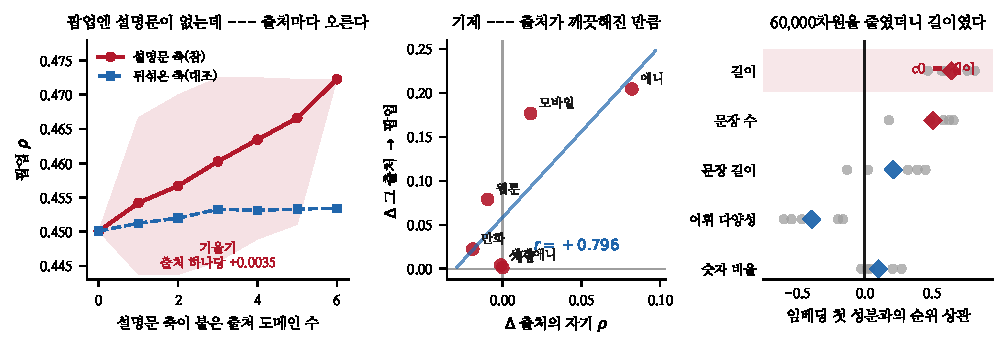
\includegraphics[width=\textwidth]{figs/bor.pdf}
\caption{왼쪽 --- 출처 수 곡선. 가운데 --- 기제. 오른쪽 --- 임베딩 첫 성분의 정체.}
\end{figure*}

\section{겹침은 새 축끼리가 아니었다}

노트 95는 세 축을 합쳐 $+$0.0351이 나와야 하는데 $+$0.0155가 나온 것을 보고
``56\%가 겹친다''고만 적었다. 무엇끼리 겹치는지 재 보았다.

\begin{table}[t]
\centering\tsize
\caption{새 축끼리의 순위 상관(둘 다 관측된 레코드).}
\begin{tabular}{lrrr}
\toprule
& 직전작$\cdot$문장수 & 표시자$\cdot$문장수 & $n$ \\
\midrule
애니 & $+$0.188 & $-$0.055 & 1,199 \\
모바일 & \textbf{$+$0.283} & $+$0.035 & 722 \\
웹툰 & $+$0.027 & $+$0.096 & 1,101 \\
만화 & $-$0.002 & $+$0.043 & 624 \\
세계애니 & $+$0.010 & $+$0.089 & 2,723 \\
\bottomrule
\end{tabular}
\end{table}

\begin{table}[t]
\centering\tsize
\caption{새 축과 \emph{기존} 다섯 공통 축의 상관. 절댓값 0.13 이상만.}
\begin{tabular}{llr}
\toprule
& 기존 축 & $r$ \\
\midrule
직전작 · 모바일 & 입장료 & \textbf{$-$0.495} \\
직전작 · 애니 & 매장 노출 & $-$0.267 \\
직전작 · 모바일 & 미디어 홍보 & $+$0.262 \\
직전작 · 모바일 & 굿즈 규모 & $+$0.220 \\
직전작 · 모바일 & 타깃 폭 & $+$0.203 \\
문장 수 · 세계애니 & 타깃 폭 & $+$0.201 \\
문장 수 · 모바일 & 굿즈 규모 & $+$0.200 \\
문장 수 · 웹툰 & 타깃 폭 & $+$0.197 \\
\bottomrule
\end{tabular}
\end{table}

\claimx{노트 95의 겹침은 \emph{새 축끼리}가 아니라 \textbf{새 축과 기존 축}
사이다. 직전작과 문장 수는 다섯 중 셋에서 상관이 0.03 아래인데, 둘 다 기존
다섯 축과는 0.20$\sim$0.50으로 붙는다.}{상관은 선형 관계만 잡는다. 인자 공간에
들어가면 주성분 둘로 줄어들므로 여기서 안 겹쳐도 거기서 겹칠 수 있다.}

이것이 실무적으로 뜻하는 바는 분명하다 --- \textbf{서로 다른 새 축을 여럿
모으는 전략은 안 통한다.} 새 축은 서로가 아니라 이미 있는 것과 싸운다.

\section{60,000차원을 줄였더니 길이였다}

노트 95는 손으로 고른 특징 다섯을 썼다. 문장 임베딩 모형을 못 내려받으므로
\textbf{문자 $n$-그램 TF-IDF $+$ SVD} 로 대신했다. 한국어 · 일본어 · 영어가
섞여 형태소 분석이 안 되는데 문자 2--4 그램은 언어를 안 가린다.

\begin{table}[t]
\centering\tsize
\caption{임베딩을 만든 코퍼스. 여섯 도메인 전부 덮개율 100\%.}
\begin{tabular}{lrl}
\toprule
& 건수 & 출처 \\
\midrule
애니 & 2,068 & 라프텔 줄거리 \\
모바일 & 2,000 & 앱스토어 소개문 \\
웹툰 & 2,817 & 네이버 시놉시스 \\
만화 & 1,788 & AniList \\
세계애니 & 2,948 & AniList \\
\textbf{게임} & \textbf{482} & \textbf{스팀(이번에 붙임)} \\
\midrule
합 & \textbf{12,103} & 어휘 60,000 \\
\bottomrule
\end{tabular}
\end{table}

게임은 캐시에 스팀 \texttt{about\_the\_game} 이 이미 1,494건 있었다. 축
레코드 482건과 \textbf{482/482로 전부 맞는다.} 여섯째 설명문 도메인이 공짜로
생겼다.

\begin{table}[t]
\centering\tsize
\caption{첫 성분 c0 과 손 특징 다섯의 순위 상관.}
\begin{tabular}{lrrrrr}
\toprule
& 애니 & 모바일 & 웹툰 & 만화 & 세계애니 \\
\midrule
\textbf{길이} & \textbf{$+$.61} & \textbf{$+$.47} & \textbf{$+$.57} &
\textbf{$+$.76} & \textbf{$+$.82} \\
문장 수 & $+$.63 & $+$.18 & $+$.58 & $+$.49 & $+$.66 \\
문장 길이 & $-$.13 & $+$.45 & $+$.02 & $+$.32 & $+$.39 \\
어휘 다양성 & $-$.20 & $-$.47 & $-$.16 & $-$.54 & $-$.60 \\
숫자 비율 & $+$.27 & $+$.04 & $+$.21 & $-$.03 & $+$.02 \\
\bottomrule
\end{tabular}
\end{table}

\claimx{60,000차원 문자 $n$-그램의 첫 주성분은 \textbf{길이}다. 다섯 도메인
전부에서 문자 수와 $+$0.47$\sim+$0.82로 붙는다. 노트 95의 손 특징 다섯은
임베딩이 잡을 것을 이미 거의 다 잡고 있었다.}{성분 하나만 봤다. c1 · c2 는
길이와 덜 붙지만 축으로 넣으면 $+$0.0069 · $+$0.0043으로 더 작다.}

\begin{table}[t]
\centering\tsize
\caption{축으로 넣은 결과. 여섯 도메인.}
\begin{tabular}{lrrr}
\toprule
& $\rho$ & $\Delta$ & 팝업 \\
\midrule
현행 & $+$0.4038 & --- & $+$0.4501 \\
\textbf{임베딩 c0} & \textbf{$+$0.4142} & $+$0.0104 & \textbf{$+$0.4723} \\
문장 수(노트 95) & $+$0.4134 & $+$0.0096 & $+$0.4481 \\
\textbf{둘 다} & $+$0.3897 & \textbf{$-$0.0141} & $+$0.4734 \\
\bottomrule
\end{tabular}
\end{table}

같은 것을 두 벌 넣으면 인자 공간이 그쪽으로 쏠려 오히려 나빠진다. 노트 95의
``작은 것들은 더해지지 않는다''가 여기서 극단적으로 나타난다.

\section{팝업엔 없는 축인데 팝업이 오른다}

임베딩은 판정치에서 $+$0.0104로 문턱(구간 반폭 0.033) 아래고 씨앗 넷 전부
보류다. \textbf{그런데 팝업이 $+$0.0222 오른다} --- 지금까지 어떤 새 축보다
크다. 팝업에는 설명문이 없고 축이 하나도 안 붙는데도 그렇다.

노트 94에서 표지 축을 넣었을 때도 팝업이 다섯 설정 모두에서 올랐고
($+$0.003$\sim+$0.007) 그때는 ``잡음과 못 가른다''고 적고 넘어갔다.
\textbf{두 번째로 같은 일이 일어났으므로 이번엔 갈랐다.}

\begin{table}[t]
\centering\tsize
\caption{여섯 출처 중 $k$개에만 축을 붙인다. 63가지 조합 전부.}
\begin{tabular}{lrrrr}
\toprule
$k$ & 조합 & $\rho$ & 팝업 & 뒤섞은 축 \\
\midrule
0 & 1 & $+$0.4038 & $+$0.4501 & $+$0.4501 \\
1 & 6 & $+$0.4060 & $+$0.4542 & $+$0.4513 \\
2 & 15 & $+$0.4078 & $+$0.4567 & $+$0.4520 \\
3 & 20 & $+$0.4097 & $+$0.4603 & $+$0.4533 \\
4 & 15 & $+$0.4114 & $+$0.4635 & $+$0.4531 \\
5 & 6 & $+$0.4128 & $+$0.4666 & $+$0.4533 \\
6 & 1 & $+$0.4142 & \textbf{$+$0.4723} & $+$0.4534 \\
\midrule
\multicolumn{2}{l}{기울기(출처 하나당)} & $+$0.0017 &
\textbf{$+$0.0035} & $+$0.0005 \\
\bottomrule
\end{tabular}
\end{table}

\claimx{대상에 없는 축이 대상을 돕고, 그 도움은 \textbf{축을 받은 출처 수에
비례한다} --- 출처 하나당 팝업 $+$0.0035. 63가지 조합에서 단조이고 거의
직선이다. 같은 자리에 뒤섞은 축을 넣으면 기울기가 $+$0.0005로 평평해지므로
\textbf{차원이 아니라 정보다.}}{뒤섞은 축도 절편은 $+$0.003쯤 올린다 --- 축
하나를 더하는 것 자체에 작은 이득이 있다. 기울기만 정보의 몫이다.}

\begin{table}[t]
\centering\tsize
\caption{기제 --- 출처의 자기 $\rho$와 그 출처의 팝업 전이.}
\begin{tabular}{lrrrr}
\toprule
& \multicolumn{2}{c}{자기 $\rho$} & \multicolumn{2}{c}{$\to$ 팝업} \\
& 전 & 후 & 전 & 후 \\
\midrule
\textbf{애니} & $+$0.292 & \textbf{$+$0.374} & $+$0.124 & \textbf{$+$0.328} \\
모바일 & $+$0.656 & $+$0.674 & $+$0.223 & $+$0.399 \\
웹툰 & $+$0.479 & $+$0.470 & $+$0.324 & $+$0.403 \\
만화 & $+$0.475 & $+$0.456 & $+$0.425 & $+$0.447 \\
세계애니 & $+$0.419 & $+$0.418 & $+$0.474 & $+$0.478 \\
게임 & $+$0.386 & $+$0.386 & $+$0.445 & $+$0.446 \\
\midrule
\multicolumn{5}{l}{두 변화량의 상관 \quad $r=+$\textbf{0.796}} \\
\bottomrule
\end{tabular}
\end{table}

\claimx{기제는 노트 74의 법칙이다 --- 출처의 자기 $\rho$가 오른 만큼 그 출처의
대상 전이가 오른다. 여기서는 그 법칙이 \emph{변화량}에도 성립한다($r=+$0.796).
설명문 축이 애니의 자기 $\rho$를 $+$0.082 올리고, 애니의 팝업 전이가 $+$0.205
오른다.}{여섯 점의 상관이다. 애니 하나가 지렛대라 그것을 빼면 $r$이 크게
떨어진다.}

\begin{quote}\fontsize{9.5}{11.5}\selectfont
\textbf{새 축을 대상에 붙일 필요가 없다.} 지금까지 새 축을 찾을 때마다 ``팝업엔
그 데이터가 없어서 못 붙인다''가 걸림돌이었다(노트 94 · 95의 한계 항목).
그런데 팝업이 얻는 이득은 \emph{출처}가 깨끗해진 데서 온다. \textbf{팝업에
없는 종류의 데이터도 값을 한다.}
\end{quote}

\section{그래서 얼마나 필요한가}

기울기가 있으면 셈이 된다. 팝업의 순 정보 기울기는 $+$0.0035에서 뒤섞은 축의
$+$0.0005를 뺀 \textbf{$+$0.0030}이다. 라벨 천장(0.734, 노트 83)까지 남은
0.284를 이것으로만 메우려면

\[ 0.284 \;/\; 0.0030 \;\approx\; \textbf{96개} \]

의 설명문 있는 출처 도메인이 필요하다. 지금 여섯이다.

\claimx{처음으로 남은 격차가 \textbf{살 수 있는 단위}로 환산됐다. 노트 93은
``축에 없는 것 0.256''이라고만 했고 노트 95는 ``$+$0.01짜리 스물다섯 개''라
했는데, 둘 다 크기를 몰랐다. 이제 안다 --- 출처 도메인 96개.}{여섯 점에 직선을
맞춰 열여섯 배 밖으로 외삽했다. 표에서 이미 감속이 보인다($k$ 1$\to$2 에서
$+$0.0025, 5$\to$6 에서 $+$0.0057이지만 3$\to$4 는 $+$0.0032). \textbf{96은
하한이 아니라 낙관적 눈금이다.}}

\section{한계}

\begin{itemize}[leftmargin=1.1em,itemsep=0.15em]
\item 임베딩이 진짜 문장 임베딩이 아니다. 문자 $n$-그램은 의미를 못 잡는다 ---
      감정 · 주제 · 고유명사는 여전히 못 쓴다.
\item 판정치는 씨앗 넷 전부 보류다($+$0.0104, 구간 $[-0.020, +0.019]$).
      팝업도 넷 다 보류다($+$0.0222, 구간 $[-0.042, +0.087]$). \textbf{채택
      안 한다.}
\item 출처 수 곡선은 한 축(c0)으로만 냈다. 다른 축도 같은 기울기인지 모른다.
\item 96개라는 셈은 여섯 점의 직선 외삽이다. 감속이 있으면 훨씬 크다.
\item 노트 94의 표지 무작위 재표집은 이번에도 안 했다.
\end{itemize}

\section{다음}

\begin{enumerate}[leftmargin=1.3em,itemsep=0.15em]
\item \textbf{기울기가 축 종류에 따라 다른가} --- 표지 축(노트 94)으로 같은
      출처 수 곡선을 낸다. 기울기가 비슷하면 ``출처 하나당''이 법칙이고,
      다르면 축의 질이 따로 있다.
\item \textbf{출처 도메인을 더 늘린다} --- 이제 늘릴 이유가 분명하다. 노트 83은
      ``도메인 추가는 정확도를 안 산다''고 했지만 그것은 축 없이 도메인만
      더할 때다. \textbf{설명문 있는 도메인은 다르다.}
\item 팝업 · 아이돌 · 도서 · 펀딩의 설명문을 찾는다. 게임이 캐시에서 공짜로
      나왔으니 남은 넷도 가능성이 있다.
\item 진짜 문장 임베딩 --- 다국어 모형을 구할 수 있으면 c0 이 길이가 아닐
      것이다.
\end{enumerate}

\vspace{0.6em}
\hrule height 0.3pt
\vspace{0.5em}
{\footnotesize
\textbf{참고문헌}\\[0.3em]
Deerwester, S. et al. (1990). Indexing by latent semantic analysis.
\emph{JASIS}, 41(6), 391--407.\\[0.15em]
Reimers, N., Gurevych, I. (2019). Sentence-BERT: sentence embeddings using
Siamese BERT-networks. \emph{EMNLP}, 3982--3992.\\[0.15em]
Ben-David, S. et al. (2010). A theory of learning from different domains.
\emph{Machine Learning}, 79(1--2), 151--175.\\[0.15em]
Lord, F. M., Novick, M. R. (1968). \emph{Statistical Theories of Mental Test
Scores}. Addison-Wesley.\\[0.15em]
Efron, B., Tibshirani, R. J. (1993). \emph{An Introduction to the Bootstrap}.
Chapman \& Hall.
}

\end{document}
